% !BIB TS-program = biber
% !BIB program = biber
\documentclass{sgreport}

\usepackage[english]{babel}
\usepackage{lipsum}
\usepackage{hyperref}
\usepackage[toc]{glossaries}
\usepackage[
backend=biber,
style=alphabetic,
sorting=ynt
]{biblatex}
\usepackage{graphicx}
\graphicspath{ {images/} }

\addbibresource{bibliography/p1_bib.bib}

\makeglossaries

\begin{document}
%------------ GLOSSARY--------------
\newglossaryentry{latex}
{
    name=\LaTeX,
    description={Is a mark up language specially suited for scientific documents}
}
\newglossaryentry{tex}
{
    name=\TeX,
    description={Is a typesetting system developed by Donald Knuth}
}
\newglossaryentry{microsoft_word}
{
    name={Microsoft Word},
    description={Is a word processor created and developed by Microsoft}
}
\newglossaryentry{google_docs}
{
    name={Google Docs},
    description={Is an online word processor created and developed by Google}
}
\newglossaryentry{libre_office}
{
    name=LibreOffice,
    description={Is an open source office suite created and developed by \acrlong{tdf}}
}
\newglossaryentry{scribus}
{
    name=Scribus,
    description={Is a is a \acrlong{dtp} application developed by \acrlong{tst}}
}
\newglossaryentry{indesign}
{
    name=InDesign,
    description={Is a desktop publishing software developed by Adobe Systems Incorporated}
}
\newglossaryentry{git}
{
    name=Git,
    description={Is a software versioning and revision control system originally created by Linus Torvalds and now developed by Junio Hamano}
}
\newglossaryentry{svn}
{
    name={Apache Subversion},
    description={Is a software versioning and revision control system developed by the \acrlong{tst}}
}
\newglossaryentry{mercurial}
{
    name=Mercurial,
    description={Is a software versioning and revision control system developed by Matt Mackall}
}
\newglossaryentry{github}
{
    name=GitHub,
    description={Is a web-based \gls{git} repository and Internet hosting service}
}
\newglossaryentry{bitbucket}
{
    name=Bitbucket,
    description={Is a web-based \gls{git} and \gls{mercurial} repository and Internet hosting service owned by Atlassian}
}
\newglossaryentry{kalarm}
{
    name=KAlarm,
    description={Is a personal alarm scheduler developed by David Jarvie}
}
\newglossaryentry{linux}
{
    name=Linux,
    description={Linux is a Unix-like computer operating system assembled under the model of free and open-source software development and distribution}
}
\newglossaryentry{unix}
{
    name=UNIX,
    description={Unix is a family of multitasking, multiuser computer operating systems that derive from the original AT\&T Unix, developed starting in the 1970s at the Bell Labs research center by Ken Thompson, Dennis Ritchie, and others.}
}
\newglossaryentry{nasl}
{
    name=NAS,
    description={The \acrlong{nas} is a network transparent, client/server audio transport system. It can be described as the audio equivalent of an X server.}
}
\newglossaryentry{continuous_integration}
{
    name={Continuous Integration},
    description={\acrlong{ci} is a development practice that requires developers
    to integrate code into a shared repository several times a day.  Each
check-in is then verified by an automated build, allowing teams to detect
problems early~\cite{thoughtworks2017}}
}
\newglossaryentry{metaclass}
{
    name=Metaclass,
    description={Class whose instances are classes}
}
\newglossaryentry{travis}
{
    name={Travis CI},
    description={Free continuous integration platform for GitHub projects}
}
\newglossaryentry{qt}
{
    name=Qt,
    description={Qt is a cross-platform application development framework for
    desktop, embedded and mobile~\cite{aboutQt2017}}
}
\newglossaryentry{python}
{
    name=Python,
    description= {Python is a widely used high-level programming language. Python has a design philosophy which emphasizes code readability, and a syntax which allows programmers to express concepts in fewer lines of code than possible in languages such as C++ or Java.}
}

%------------------- ACRONYMS ---------------------
\newacronym{gcd}{GCD}{Greatest Common Divisor}
\newacronym{tdf}{TDF}{The Document Foundation}
\newacronym{tst}{TST}{The Scribus Team}
\newacronym{dtp}{DTP}{desktop publishing}
\newacronym{asp}{ASP}{Apache Software Foundation}
\newacronym[\glslongpluralkey={version control systems}]{vcs}{VCS}{version control system}
\newacronym{mh}{MH}{Must Have}
\newacronym{p1}{P1}{First Piority}
\newacronym{p2}{P2}{Second Piority}
\newacronym{nth}{NTH}{Nice To Have}
\newacronym{lgpl}{LGPL}{Lesser General Public License}
\newacronym{gpl}{GPL}{General Public License}
\newacronym{bsd}{BSD}{Berkeley Software Distribution}
\newacronym{nas}{NAS}{Network Audio System}
\newacronym{ci}{CI}{Continuous Integration}


\university{Bern University of Applied Sciences}
\project{Project 1 - ClockAlarm}
\title{Requirements (version 1.0)}
\author{Loïc Charrière, Samuel Gauthier}
\supervisor{Claude Fuhrer}

\maketitle

\tableofcontents

\chapter{Goal of this document}

Test \cite{pohl_requirements_2011}.
\lipsum[4-7]
\chapter{Project Vision}

The goal of this project is to develop a replacement for the
program „kAlarm“ distributed with the KDE desktop
environment.

\begin{figure}[h]
\centering
\caption{kAlarm layout on KDE}
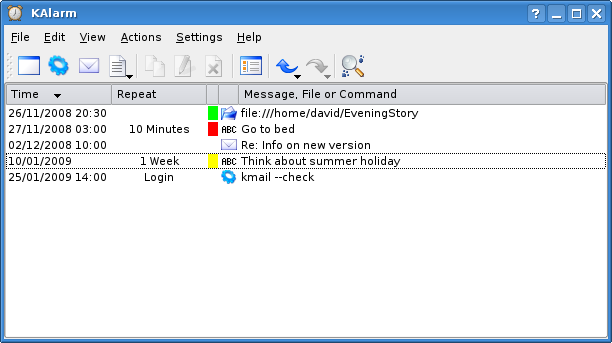
\includegraphics[width=0.7\textwidth]{kalarm.png}
\end{figure}

The program kAlarm allows the user to define some events
(possibly recurrent) and display alarms using pop-up windows
on the screen at times defined by the event. The project should
develop an alternative to this tool, which is platform
independent and open-source.
\chapter{Project goals}
\lipsum[4-7]
\chapter{System and Context Boundaries}
\lipsum[4-7]
\chapter{Requirements}
\lipsum[4-7]
As an [actor] I want [action] so that [achievement].
\newcounter{counter}

\subsection{As a User}
\subsubsection{Alerts functionality}
\begin{enumerate}
	\item I want to registrate some alerts so that the software warns me when they occure
	\item I want to be able to chose a different color, font and sound for every alert
	\item I want to edit the existing alerts when needed
	\item I want to delete the existing alerts when needed
	\item I want to postpone an alarm so that i'm notified again later (snooze)
	\item I want to mute an alert so that i'm not notified
	\setcounter{counter}{\value{enumi}}
\end{enumerate}
\subsubsection{Managing alerts}
\begin{enumerate}
	\setcounter{enumi}{\value{counter}}
	\item I want to create categories of alerts, so that I can sort my alerts
	\item I want to edit my categories, in a way my alerts remain categorised
	\item I want to delete categories of alerts, so that my list of categories stay concise
	\item I want to assign color identity to my different categories, some that I can easily find them
	\item I want to personalize the default color, font and sound of my alarms in the software configurations
	\item I want to mute an alert catogory so that i'm not notified by any alert in this category
	\setcounter{counter}{\value{enumi}}
\end{enumerate}
\subsubsection{Persistence}
\begin{enumerate}
	\setcounter{enumi}{\value{counter}}
	\item I want to retrieve the correct state of my alerts after turning my computer down and back on
	\item I want to be alerted at any times, as soon as I'm loged on my computer session
	\setcounter{counter}{\value{enumi}}
\end{enumerate}
\subsubsection{Exportability}
\begin{enumerate}
	\setcounter{enumi}{\value{counter}}
	\item I want to export my alerts so that I can't import then on an other computer with ClockAlarm installed
	\item I want to import an alerts file, so that I can retrieve previously exported alerts
	\item I want to load configuration files, so that I can use predifined color and sound themes
	\setcounter{counter}{\value{enumi}}
\end{enumerate}
\subsubsection{Pivacy}
\begin{enumerate}
	\setcounter{enumi}{\value{counter}}
	\item I want my alerts to remain private, so that nobody except me knows about them
\end{enumerate}
\chapter{Use Cases}

\section{Use Case \arabic{subsection}: Template}

\subsubsection{Scope}

\subsubsection{Primary actor}

\subsubsection{Precondition}

\subsubsection{Postcondition}

\subsubsection{Main success scenario}

\subsubsection{Extension}


%\clearpage

\printglossaries

\printbibliography[
heading=bibintoc,
title={Bibliography}
]

\end{document} 